% Options for packages loaded elsewhere
\PassOptionsToPackage{unicode}{hyperref}
\PassOptionsToPackage{hyphens}{url}
%
\documentclass[
  ignorenonframetext,
]{beamer}
\usepackage{pgfpages}
\setbeamertemplate{caption}[numbered]
\setbeamertemplate{caption label separator}{: }
\setbeamercolor{caption name}{fg=normal text.fg}
\beamertemplatenavigationsymbolsempty
% Prevent slide breaks in the middle of a paragraph
\widowpenalties 1 10000
\raggedbottom
\setbeamertemplate{part page}{
  \centering
  \begin{beamercolorbox}[sep=16pt,center]{part title}
    \usebeamerfont{part title}\insertpart\par
  \end{beamercolorbox}
}
\setbeamertemplate{section page}{
  \centering
  \begin{beamercolorbox}[sep=12pt,center]{part title}
    \usebeamerfont{section title}\insertsection\par
  \end{beamercolorbox}
}
\setbeamertemplate{subsection page}{
  \centering
  \begin{beamercolorbox}[sep=8pt,center]{part title}
    \usebeamerfont{subsection title}\insertsubsection\par
  \end{beamercolorbox}
}
\AtBeginPart{
  \frame{\partpage}
}
\AtBeginSection{
  \ifbibliography
  \else
    \frame{\sectionpage}
  \fi
}
\AtBeginSubsection{
  \frame{\subsectionpage}
}
\usepackage{amsmath,amssymb}
\usepackage{iftex}
\ifPDFTeX
  \usepackage[T1]{fontenc}
  \usepackage[utf8]{inputenc}
  \usepackage{textcomp} % provide euro and other symbols
\else % if luatex or xetex
  \usepackage{unicode-math} % this also loads fontspec
  \defaultfontfeatures{Scale=MatchLowercase}
  \defaultfontfeatures[\rmfamily]{Ligatures=TeX,Scale=1}
\fi
\usepackage{lmodern}
\usetheme[]{AnnArbor}
\usecolortheme{dolphin}
\usefonttheme{structurebold}
\ifPDFTeX\else
  % xetex/luatex font selection
\fi
% Use upquote if available, for straight quotes in verbatim environments
\IfFileExists{upquote.sty}{\usepackage{upquote}}{}
\IfFileExists{microtype.sty}{% use microtype if available
  \usepackage[]{microtype}
  \UseMicrotypeSet[protrusion]{basicmath} % disable protrusion for tt fonts
}{}
\makeatletter
\@ifundefined{KOMAClassName}{% if non-KOMA class
  \IfFileExists{parskip.sty}{%
    \usepackage{parskip}
  }{% else
    \setlength{\parindent}{0pt}
    \setlength{\parskip}{6pt plus 2pt minus 1pt}}
}{% if KOMA class
  \KOMAoptions{parskip=half}}
\makeatother
\usepackage{xcolor}
\newif\ifbibliography
\usepackage{graphicx}
\makeatletter
\def\maxwidth{\ifdim\Gin@nat@width>\linewidth\linewidth\else\Gin@nat@width\fi}
\def\maxheight{\ifdim\Gin@nat@height>\textheight\textheight\else\Gin@nat@height\fi}
\makeatother
% Scale images if necessary, so that they will not overflow the page
% margins by default, and it is still possible to overwrite the defaults
% using explicit options in \includegraphics[width, height, ...]{}
\setkeys{Gin}{width=\maxwidth,height=\maxheight,keepaspectratio}
% Set default figure placement to htbp
\makeatletter
\def\fps@figure{htbp}
\makeatother
\setlength{\emergencystretch}{3em} % prevent overfull lines
\providecommand{\tightlist}{%
  \setlength{\itemsep}{0pt}\setlength{\parskip}{0pt}}
\setcounter{secnumdepth}{-\maxdimen} % remove section numbering
\ifLuaTeX
  \usepackage{selnolig}  % disable illegal ligatures
\fi
\usepackage{bookmark}
\IfFileExists{xurl.sty}{\usepackage{xurl}}{} % add URL line breaks if available
\urlstyle{same}
\hypersetup{
  pdftitle={Winning the Lottery (BUS124B)},
  pdfauthor={Mario Arce Acosta},
  hidelinks,
  pdfcreator={LaTeX via pandoc}}

\title{Winning the Lottery (BUS124B)}
\author{Mario Arce Acosta}
\date{2024-06-14}

\begin{document}
\frame{\titlepage}

\begin{frame}{Next Steps}
\phantomsection\label{nextsteps}
\#nextsteps \{ color: blue; \}

.emphasized \{ font-size: 1.2em; \} - (Primary) Are certain industries
associated with higher H-1B visa petition approval ratios? - (Relevance)
How can the findings influence nonprofits for immigration, like the
California Immigrant Policy Center, in their decision-making? -
(Secondary) What are some trends in immigration regarding H-1B visas and
LPR status?
\end{frame}

\begin{frame}[fragile]{Data Methodology}
\phantomsection\label{data-methodology}
\begin{itemize}
\tightlist
\item
  I exported two datasets from the US Citizenship and Immigration
  Services (USCIS); one from their H-1B Data Hub webpage, the other
  dataset is yearbook of people who obtained Lawful Permanent Residency
  (LPR) status
\item
  H-1B Data: I exported data from the USCIS H-1B Employer Data Hub by
  splitting exports into sections of a few years since the final dataset
  would include over 900,000 observations
\item
  LPR Data: I exported this data from the USCIS
\end{itemize}

\begin{verbatim}
## Registered S3 method overwritten by 'quantmod':
##   method            from
##   as.zoo.data.frame zoo
\end{verbatim}

\begin{verbatim}
## 
## Please cite as:
\end{verbatim}

\begin{verbatim}
##  Hlavac, Marek (2022). stargazer: Well-Formatted Regression and Summary Statistics Tables.
\end{verbatim}

\begin{verbatim}
##  R package version 5.2.3. https://CRAN.R-project.org/package=stargazer
\end{verbatim}

\begin{verbatim}
## Warning: One or more parsing issues, call `problems()` on your data frame for details,
## e.g.:
##   dat <- vroom(...)
##   problems(dat)
\end{verbatim}

\begin{verbatim}
## Rows: 927193 Columns: 11
\end{verbatim}

\begin{verbatim}
## -- Column specification --------------------------------------------------------
## Delimiter: ","
## chr (4): Employer (Petitioner) Name, Industry (NAICS) Code, Petitioner City,...
## dbl (5): Fiscal Year, Tax ID, Petitioner Zip Code, Initial Denial, Continuin...
## num (2): Initial Approval, Continuing Approval
## 
## i Use `spec()` to retrieve the full column specification for this data.
## i Specify the column types or set `show_col_types = FALSE` to quiet this message.
\end{verbatim}

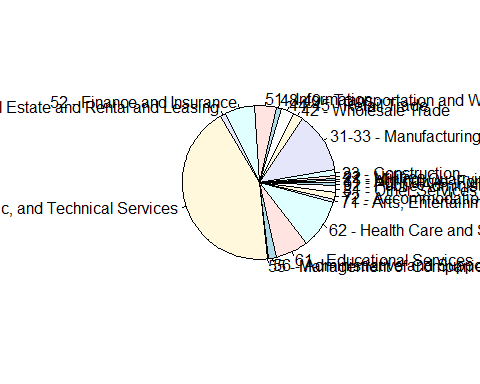
\includegraphics{BUS124B_H-1B_Project_Mario_files/figure-beamer/H1B_Data Clean & Prepare-1.pdf}
\end{frame}

\begin{frame}{H-1B (aggregated by year) Summary Table}
\phantomsection\label{h-1b-aggregated-by-year-summary-table}
\begin{longtable}[t]{lllllllll}
\toprule
 & Year & Initial\_Approval & Initial\_Denial & Continuing\_Approval & Continuing\_Denial & IAppovals ratio & CApproval ratio & Approvals ratio\\
\midrule
 & Min.   :2009 & Min.   : 83965 & Min.   : 2988 & Min.   :108879 & Min.   : 4009 & Min.   :0.2970 & Min.   :0.4706 & Min.   :0.8455\\
 & 1st Qu.:2012 & 1st Qu.:100891 & 1st Qu.: 7458 & 1st Qu.:157414 & 1st Qu.: 5222 & 1st Qu.:0.3517 & 1st Qu.:0.4959 & 1st Qu.:0.9047\\
 & Median :2016 & Median :116548 & Median :10108 & Median :209903 & Median : 6310 & Median :0.3755 & Median :0.5480 & Median :0.9171\\
 & Mean   :2016 & Mean   :114435 & Mean   :12334 & Mean   :209127 & Mean   :10351 & Mean   :0.3725 & Mean   :0.5405 & Mean   :0.9131\\
 & 3rd Qu.:2019 & 3rd Qu.:130058 & 3rd Qu.:14812 & 3rd Qu.:270906 & 3rd Qu.:14453 & 3rd Qu.:0.4047 & 3rd Qu.:0.5794 & 3rd Qu.:0.9286\\
\addlinespace
 & Max.   :2022 & Max.   :140715 & Max.   :32279 & Max.   :309745 & Max.   :25978 & Max.   :0.4428 & Max.   :0.6076 & Max.   :0.9661\\
\bottomrule
\end{longtable}
\end{frame}

\begin{frame}{H-1B (Panel Data) Summary Table}
\phantomsection\label{h-1b-panel-data-summary-table}
\begin{longtable}[t]{llllllllllllllllll}
\toprule
 & Year & Employer (Petitioner) Name & Tax ID & Industry (NAICS) Code & Petitioner City & Petitioner State & Petitioner Zip Code & Initial\_Approval & Initial\_Denial & Continuing\_Approval & Continuing\_Denial & IAppovals ratio & CApproval ratio & Approvals ratio & Professional & Health & Finance\\
\midrule
 & Min.   :2009 & Length:726901 & Min.   :   0 & Length:726901 & Length:726901 & Length:726901 & Min.   :  604 & Min.   :   0.000 & Min.   :  0.0000 & Min.   :    0.000 & Min.   :  0.0000 & Min.   :0.0000 & Min.   :0.0000 & Min.   :0.0000 & Min.   :0.0000 & Min.   :0.00000 & Min.   :0.0000\\
 & 1st Qu.:2012 & Class :character & 1st Qu.:2403 & Class :character & Class :character & Class :character & 1st Qu.:15601 & 1st Qu.:   0.000 & 1st Qu.:  0.0000 & 1st Qu.:    0.000 & 1st Qu.:  0.0000 & 1st Qu.:0.0000 & 1st Qu.:0.0000 & 1st Qu.:1.0000 & 1st Qu.:0.0000 & 1st Qu.:0.00000 & 1st Qu.:0.0000\\
 & Median :2016 & Mode  :character & Median :4919 & Mode  :character & Mode  :character & Mode  :character & Median :48066 & Median :   0.000 & Median :  0.0000 & Median :    1.000 & Median :  0.0000 & Median :0.0000 & Median :0.6316 & Median :1.0000 & Median :0.0000 & Median :0.00000 & Median :1.0000\\
 & Mean   :2016 & NA & Mean   :4936 & NA & NA & NA & Mean   :49262 & Mean   :   1.994 & Mean   :  0.2207 & Mean   :    3.698 & Mean   :  0.1868 & Mean   :0.3729 & Mean   :0.5406 & Mean   :0.9134 & Mean   :0.2335 & Mean   :0.04198 & Mean   :0.6768\\
 & 3rd Qu.:2019 & NA & 3rd Qu.:7442 & NA & NA & NA & 3rd Qu.:84095 & 3rd Qu.:   1.000 & 3rd Qu.:  0.0000 & 3rd Qu.:    1.000 & 3rd Qu.:  0.0000 & 3rd Qu.:1.0000 & 3rd Qu.:1.0000 & 3rd Qu.:1.0000 & 3rd Qu.:0.0000 & 3rd Qu.:0.00000 & 3rd Qu.:1.0000\\
\addlinespace
 & Max.   :2022 & NA & Max.   :9999 & NA & NA & NA & Max.   :99929 & Max.   :9179.000 & Max.   :947.0000 & Max.   :25201.000 & Max.   :947.0000 & Max.   :1.0000 & Max.   :1.0000 & Max.   :1.0000 & Max.   :1.0000 & Max.   :1.00000 & Max.   :1.0000\\
 & NA & NA & NA's   :8709 & NA & NA & NA & NA's   :153 & NA & NA's   :2 & NA & NA & NA's   :3 & NA's   :3 & NA's   :3 & NA & NA & NA\\
\bottomrule
\end{longtable}
\end{frame}

\begin{frame}{Time Series Plots of H-1B petitions (2009-2022)}
\phantomsection\label{time-series-plots-of-h-1b-petitions-2009-2022}
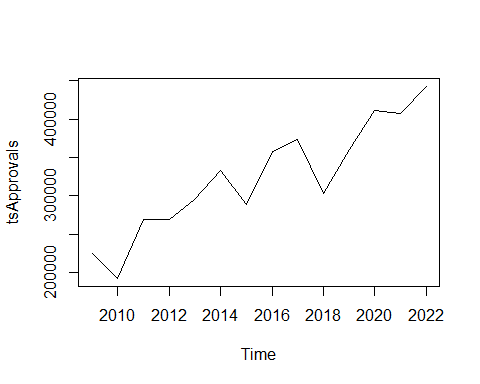
\includegraphics{BUS124B_H-1B_Project_Mario_files/figure-beamer/EDA H-1B-1.pdf}
\end{frame}

\begin{frame}[fragile]{Model Creation and Residual Plots for H-1B data}
\phantomsection\label{model-creation-and-residual-plots-for-h-1b-data}
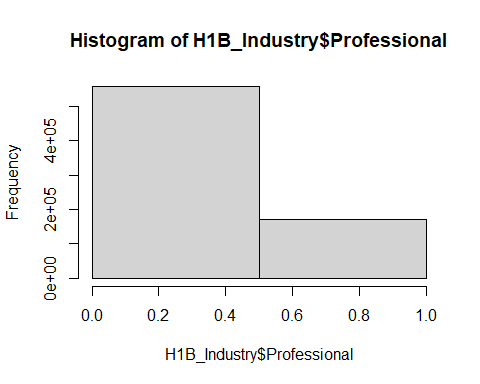
\includegraphics{BUS124B_H-1B_Project_Mario_files/figure-beamer/Create Models-1.pdf}
\includegraphics{BUS124B_H-1B_Project_Mario_files/figure-beamer/Create Models-2.pdf}
\includegraphics{BUS124B_H-1B_Project_Mario_files/figure-beamer/Create Models-3.pdf}
\includegraphics{BUS124B_H-1B_Project_Mario_files/figure-beamer/Create Models-4.pdf}

\begin{verbatim}
## 
## ==================================================================================================================================================
##                                                                               Dependent variable:                                                 
##                               --------------------------------------------------------------------------------------------------------------------
##                                                                                `Approvals ratio`                                                  
##                                            (1)                         (2)                          (3)                           (4)             
## --------------------------------------------------------------------------------------------------------------------------------------------------
## Professional, Health, Finance           0.023***                    -0.003***                                                                     
##                                          (0.001)                     (0.001)                                                                      
##                                                                                                                                                   
## Health                                  -0.067***                                                -0.059***                                        
##                                          (0.002)                                                  (0.001)                                         
##                                                                                                                                                   
## Finance                                 -0.033***                                                                              -0.029***          
##                                          (0.001)                                                                                (0.001)           
##                                                                                                                                                   
## Constant                                0.933***                     0.914***                    0.916***                      0.933***           
##                                          (0.001)                     (0.0003)                    (0.0003)                       (0.001)           
##                                                                                                                                                   
## --------------------------------------------------------------------------------------------------------------------------------------------------
## Observations                             726,898                     726,898                      726,898                       726,898           
## R2                                        0.005                      0.00002                       0.002                         0.003            
## Adjusted R2                               0.005                      0.00002                       0.002                         0.003            
## Residual Std. Error                0.255 (df = 726894)         0.256 (df = 726896)          0.255 (df = 726896)           0.255 (df = 726896)     
## F Statistic                   1,331.512*** (df = 3; 726894) 13.691*** (df = 1; 726896) 1,580.428*** (df = 1; 726896) 2,049.790*** (df = 1; 726896)
## ==================================================================================================================================================
## Note:                                                                                                                  *p<0.1; **p<0.05; ***p<0.01
\end{verbatim}

\includegraphics{BUS124B_H-1B_Project_Mario_files/figure-beamer/Comparing H-1B models-1.pdf}

\includegraphics{BUS124B_H-1B_Project_Mario_files/figure-beamer/LPR_data Clean & Prepare-1.pdf}

\begin{verbatim}
## 
## Call:
## tslm(formula = tsLPR ~ trend)
## 
## Residuals:
##     Min      1Q  Median      3Q     Max 
## -5018.3 -3612.4  -138.1  2720.5  7520.0 
## 
## Coefficients:
##             Estimate Std. Error t value Pr(>|t|)   
## (Intercept)   1831.7     3022.5   0.606  0.56130   
## trend         2003.4      487.1   4.113  0.00338 **
## ---
## Signif. codes:  0 '***' 0.001 '**' 0.01 '*' 0.05 '.' 0.1 ' ' 1
## 
## Residual standard error: 4424 on 8 degrees of freedom
## Multiple R-squared:  0.6789, Adjusted R-squared:  0.6388 
## F-statistic: 16.91 on 1 and 8 DF,  p-value: 0.003378
\end{verbatim}

\begin{verbatim}
## 
## Call:
## tslm(formula = log(tsLPR) ~ trend)
## 
## Residuals:
##     Min      1Q  Median      3Q     Max 
## -0.3632 -0.2355 -0.0440  0.2517  0.3867 
## 
## Coefficients:
##             Estimate Std. Error t value Pr(>|t|)    
## (Intercept)   8.5513     0.2023  42.280 1.08e-10 ***
## trend         0.1422     0.0326   4.362  0.00241 ** 
## ---
## Signif. codes:  0 '***' 0.001 '**' 0.01 '*' 0.05 '.' 0.1 ' ' 1
## 
## Residual standard error: 0.2961 on 8 degrees of freedom
## Multiple R-squared:  0.704,  Adjusted R-squared:  0.667 
## F-statistic: 19.03 on 1 and 8 DF,  p-value: 0.002406
\end{verbatim}

\begin{verbatim}
## Time Series:
## Start = 1 
## End = 203 
## Frequency = 1 
##   [1]   10280.160    9711.612    9536.228    8748.660    8030.262    7994.783
##   [7]    8656.048    9310.334   12179.734   16740.414   18474.290   19928.603
##  [13]   20739.922   32662.545   40455.782   47928.547   47162.183   55886.128
##  [19]   62922.290   55719.803   59424.562   66816.993   70858.595   80970.517
##  [25]   72428.162   74284.213   86310.249  106741.974  145209.782  169604.947
##  [31]  207830.663  256475.464  293372.625  316841.737  332382.716  361017.801
##  [37]  312975.561  279213.693  270841.385  226526.769  194953.339  182559.337
##  [43]  155366.936  136352.355  148331.249  161857.274  187736.092  226985.664
##  [49]  253606.565  219176.595  259254.017  297638.712  304752.098  334768.269
##  [55]  372278.688  354596.782  316467.147  272522.803  233323.062  204866.843
##  [61]  196754.590  274905.313  393263.019  511981.714  539383.799  533146.260
##  [67]  491806.182  444525.227  458200.359  484806.951  472692.966  467475.676
##  [73]  495328.673  520628.971  496359.280  433140.796  380759.357  369511.650
##  [79]  327907.755  298325.129  302342.090  346211.063  388723.144  466729.101
##  [85]  583824.171  652537.919  764726.244  865528.871  991474.909  928893.437
##  [91]  875761.206  925503.844  911428.791  889451.754  981983.827 1052932.679
##  [97]  835062.875  674191.813  560555.169  425574.018  340241.413  367169.289
## [103]  498586.902  441877.632  466190.042  538401.829  465175.481  416969.236
## [109]  392430.966  366878.176  340718.123  311012.686  246850.580  183468.206
## [115]  135348.144  103584.701   82996.091   68995.964   63370.374   64727.762
## [121]   70208.833   70372.983   64793.888   53990.022   44910.515   40002.661
## [127]   39437.563   60222.594   86343.416  111611.391  134623.074  168992.252
## [133]  180009.676  205662.773  195094.141  199018.999  210650.299  243942.709
## [139]  268819.997  264153.498  263113.248  263798.674  266062.272  271372.490
## [145]  281838.743  284961.520  288482.164  298849.515  317786.260  358784.782
## [151]  358723.048  363103.933  365316.153  371126.807  379343.265  383715.986
## [157]  384214.590  418678.113  430701.179  478433.825  453176.878  474512.314
## [163]  510662.820  517551.174  527301.422  531654.295  542602.707  559829.995
## [169]  571847.696  592697.187  741939.631  980119.342 1234062.039 1155876.927
## [175] 1080288.649  997399.954  914233.068  914631.148  879595.903  811678.932
## [181]  761611.353  785428.547  867470.583  925036.208  858587.946  888376.462
## [187]  958540.623 1050817.136 1051296.495 1068045.347 1086877.143 1073601.500
## [193] 1070133.050 1058582.435 1038173.604 1031676.923 1037483.146 1081289.702
## [199] 1095052.892 1095520.324 1076393.727  965684.209  897979.546
\end{verbatim}

\begin{verbatim}
##                     ME     RMSE      MAE       MPE     MAPE
## Test set -1.818268e-13 3957.349 3405.915 -7.423898 32.63382
\end{verbatim}

\begin{verbatim}
##                ME     RMSE      MAE      MPE     MAPE
## Test set 12840.78 14616.87 12840.78 99.90886 99.90886
\end{verbatim}
\end{frame}

\end{document}
